%\documentclass[twoside, a4paper, DIV=11, bibliography=totocnumbered]{scrreprt}
\documentclass[twoside, a4paper, DIV=11, open=any, bibliography=totoc]{scrbook}

\usepackage{url}
\usepackage{hyperref}
\usepackage{graphicx}
\usepackage[all]{hypcap}
\usepackage[utf8]{inputenc}
\usepackage[ngerman]{babel}
\usepackage[skipabove=\baselineskip,skipbelow=\baselineskip,outermargin=30pt,innermargin=30pt]{mdframed}

\usepackage{mdframed}

\usepackage{blindtext} % remove this one, only for template/demonstration

\newcommand{\Quote}[1]{\glqq #1\grqq{}}

\hypersetup
{
 pdfauthor={Vorname Name},
 pdftitle={Seminararbeit ... },
 pdfkeywords={...},
 colorlinks=true,
 citecolor=black,
 filecolor=black,
 linkcolor=black,
 urlcolor=black
}

\KOMAoption{headings}{normal}

\tolerance=4000
\emergencystretch=20pt

\begin{document}

%*************************************************************************
\begin{titlepage}
    \subject{LVA: "`Technik für Menschen 2040"'}
    \title{Literaturarbeit, Übungskritik \& Szenario 2040}
    \author{
        Florian Schager\\
        \small 11819578
    }
    \date{\today}
    \titlehead{Sommersemester 2021}
\end{titlepage}
\maketitle
%*************************************************************************



\tableofcontents


%*************************************************************************
%*************************************************************************
\chapter{Über den Autor} \label{chap:Autor}

\section{Stammdaten} \label{sec:stammdaten}

Name: Florian Schager\\
MatNr: 11819578\\
Studium: Bachelorstudium Technische Mathematik \\
Semester: 6.Semester \\

\section{Freiwillige Selbstbeschreibung} \label{sec:selbstbeschreibung}

\textit{Freiwillig: ein paar Worte der Selbstbeschreibung}

\begin{itemize}
    \item Was interessiert mich an meinem Studium, warum habe ich es gewählt?
    \item Welche Themen und Gedanken beschäftigen mich?
    \item Warum habe ich diese LVA gewählt?
    \item Interesse auch in Zukunft vernetzt zu bleiben, um wichtige Zukunftsthemen zu diskutieren?
    \item Interesse an Bakk-/Diplomarbeit, Praktikum etc.?
    \item Kontaktinformation, Email, Webseite, Twitter
\end{itemize}


etc.

%*************************************************************************
%*************************************************************************
\chapter{Literaturarbeit} \label{chp:LitKrit}

\section{Literatur-Gruppe} \label{sec:litgruppe}

Die Literaturarbeit wurde in Gruppe 11 durchgeführt. Mitglieder dieser Gruppe waren:

\begin{itemize}
    \item 01325974 – Natasa, Nitic: Julien Offray de la Mettrie, Der Mensch eine Maschine
    \item 01427388 – Chang Hyuk, Kong: ???
    \item 01326815 – Bianca, Träger: Richard David Precht, Künstliche Intelligenz und der Sinn des Lebens
    \item 11819578 – Florian, Schager: Nick Bostrom, Superintelligence
\end{itemize}


\section{Literatur} \label{sec:litlit}

Im Rahmen der Literaturkritik wurde das Buch Superintelligence von Nick Bostrom
aus dem Jahr 2014 gelesen.

\section{Synopsis} \label{sec:litsynops}

Der Autor baut strukturiert sein Argument dafür auf, dass die potentielle zukünftige
Entwicklung von \Quote{Superintelligence}, also übermenschlicher künstlicher Intelligenz,
eine existentielle Gefahr für die Menschheit darstellt. Daraus leitet er den
Handlungsaufruf ab, bereits jetzt Forschung zur Sicherheit dieser Technologien
priorisiert voranzutreiben.

Im ersten Teil des Buches argumentiert der Autor anhand der geschichtlichen Entwicklungen,
sowie möglichen zukünftigen Innovationen, dass die Entwicklung von human-level artificial
general intelligence (AGI) zwar wahrscheinlich nicht unmittelbar bevorsteht, aber
eine reale Chance besteht, dass innerhalb des 21.Jahrhunderts human-level AGI
erreicht werden könnte. Er beschreibt dabei in dem Zusammenhang auch die große
Uneinigkeit unter Experten, was Zukunftseinschätzungen zum Thema AGI angeht.
Des weiteren beschreibt er unterschiedliche mögliche Wege zu einer potentiellen
Superintelligenz
\footnote{\begin{itemize}
  \item Künstliche Intelligenz
  \item Biologische Verbesserung menschlicher Gehirne
  \item Gehirn-Emulation
\end{itemize}}
und welche möglichen \Quote{Takeoff}-Szenarien damit einhergehen könnten.
Als \Quote{Takeoff} bezeichnet er dabei den Prozess von human-level AGI zu
vollständiger Superintelligenz, einer KI, die die menschlichen intellektuellen Fähigkeiten
um Größenordnungen übersteigt, und somit das Potential hätte, die Welt sich ihrem
Willen zu unterwerfen. In einem schnellen Szenario, welches er für durchaus
wahrscheinlich hält, könnte dieser Prozess innerhalb
weniger Stunden passieren, während ein langsamer \Quote{Takeoff} sich über Monate
bis Jahre hinziehen könnte.

Darauf aufbauend untermauert er seine These, dass eine Maschine, welche der Menschheit
in genereller Intelligenz deutlich überlegen ist, definit in der Lage wäre,
die Weltherrschaft an sich zu reißen. Dabei stellt er auch das Konzept von
\Quote{instrumental convergence} vor: Wir können zwar in der Theorie eine KI
mit belieben Werten und Zielen (\Quote{final goals}) versehen, die wenig miteinander gemein haben.
Dennoch können wir heute schon \Quote{instrumental goals} identifizieren, welche
instrumentell hilfreich für eine breite Anzahl an möglichen \Quote{final goals} sind.
Ein wichtiges Beispiel dafür ist das Ziel der \Quote{goal-integrity}. Eine hinreichend
intelligenter Agent wird mit allen Mitteln verhindern wollen, dass seine finalen Ziele
geändert werden, da dies mit sehr hoher Wahrscheinlichkeit dazu führen würde,
dass seine momentanen finalen Ziele nicht erreicht werden würden. Weitere Beispiele
für allgemeine \Quote{instrumental goals} sind der Erwerb von Ressourcen und der
Drang zur Selbstverbesserung.
Daher schließt er, dass die einzige Chance eine sichere Superintelligenz zu entwickeln,
daraus besteht, bereits im Vorhinein

Im zweiten Teil beschäftigt sich Bostrom mit dem Problem, wie wir eine kontrollierte
Intelligenzexplosion starten können, ohne die Menschheit dabei in die Sklaverei
unter einer algorithmischen Wirtschaft zu verkaufen. Dabei geht es ihm besonders
darum, wie wir eine KI mit menschlich verträglichen Werten und Zielen versehen können.
Einerseits geht er hier auf mögliche technische Pitfalls bei der Implementierung ein,
andererseits geht er aber auch auf das Problem ein, welche Ziele wir uns überhaupt
für eine KI wünschen würden, wenn wir in der Lage wären, diese uneingeschränkt und
ohne Informationsverlust der KI anzueignen.
Insbesondere argumentiert er anhand von Beispielen, dass eine direkte Spezifikation
unserer Ziele höchstwahrscheinlich katastrophale Folgen haben könnte.
Zum Beispiel könnten wir unserer KI das Ziel geben das menschliche Glück zu maximieren.
Die Superintelligenz könnte daraufhin Elektroden in unser Gehirn implantieren, welche
permanent unser Lustzentrum stimulieren würden.

Er stellt in diesem Zusammenhang mehrere interessante Konzepte vor.
Sie alle bauen darauf auf, dass wir der KI nicht selbst direkt unsere fehlerhaften
Ziele mitgeben, sondern stattdessen der KI das Ziel geben unsere implizit definierten
Werte zu lernen. Im Grunde genommen wollen wir der KI das Ziel \Quote{Do what I mean}
anstatt \Quote{Do what I say} mitgeben.
Eine Beispiel für dieses Konzept stellt er mit \Quote{Coherent extrapolated volition},
kurz CEV vor. Die Idee dahinter ist, dass die KI unsere Wünsche, wenn wir mehr wüssten,
schneller denken und bessere Entwicklungsmöglichkeiten hätten, lernt.
Dabei soll die KI nur dann handeln, wenn es eine breite Mehrheit unter allen
menschlichen extrapolierten Wünschen gibt.
Dieses System der Zielsetzung soll im Idealfall sicherstellen, dass die Menschheit
trotz der Existenz einer super-intelligenten KI, welche unter anderen Zielsetzungen
das Potential hätte, die Weltherrschaft an sich zu reißen, immer noch die Kontrolle
über ihr eigenes Schicksal behält.
Eine Möglichkeit in diesem Szenario wäre dann, dass die Menschheit über ihren
extrapolierten Willen, dass die KI auf unserer Welt keine Rolle spielen sollte,
indirekt dafür sorgt, dass sich die KI friedlich selbst herunterfährt.

\section{Erkenntnisse} \label{sec:literkenntnis}

Ich fand das Thema künstliche Intelligenz bereits bevor ich das Buch gelesen hatte, spannend.
Der strukturierte, aufbauende Stil des Buches hat mir einen tieferen Einblick in
die Möglichkeiten, Gefahren und Wege zu dieser Technologie geliefert.
Für mich wirft das Buch interessante Fragen, vor allem im Bereich der Zielsetzung von KIs auf,
unter anderem:

\section{Kritik} \label{sec:litkritik}

Bostrom geht das Thema Superintelligenz aus einer relativ technischen Perspektive
an. Oftmals wird mit physikalischen Limitationen argumentiert, er referenziert
zahlreiche Quellen und scheut sich nicht auf fachliche Details einzugehen, um seine
Argumente zu untermauern. Während es ihm weitestgehend gut gelingt, den Inhalt seiner
Thesen verständlich zu vermitteln, erschwert die sprachliche Struktur und der
verschachtelte Satzbau oftmals die Lesbarkeit.
Besonders gestört hat mich das bei seinen teilweise
langatmig gestalteten Szenarien, welche wohl seine Thesen illustrieren sollten,
sich allerdings meistens eher wie ein sehr langweiliges Science-Fiction Buch lesen.
Er gibt ja selbst zu, dass die von ihm konstruierten Szenarien eine reine Spekulation
darstellen und keinesfalls Prognosecharakter haben. Daher erschließt sich mir
der Sinn eher weniger, dass er sich beispielsweise mit Möglichkeiten in der
Organisationsstruktur von Unternehmen bestehend aus simulierten Gehirnen näher auseinandersetzt.

\section{Gegenüberstellung} \label{sec:litgegenueber}

In der Gegenüberstellung der Bücher in der Gruppe wurden folgende Aspekte diskutiert, erkannt usw. \ldots

\section{Fragen und Diskussion in der VU} \label{sec:fragenvu}

Folgende Fragen wurden für die VU vorbereitet und diskutiert:

\begin{itemize}
  \item Was können wir heute tun, um die Sicherheit einer potentiellen Intelligenzexplosion
  in der Zukunft zu erhöhen?
  \item Welche Ziele wollen wir einer potentiellen super-intelligenten KI mitgeben?
  \item Sollten wir versuchen, die Entwicklung von AGI aktiv zu verhindern?
  \item Wie können wir eine globale Zusammenarbeit zu diesem Thema fördern,
  um ein gefährliches Rennen um die erste KI zu vermeiden?
\end{itemize}


%*************************************************************************
%*************************************************************************
\chapter{Podcast-Episoden-Kritik} \label{chap:podkrit}


\section{Podcast: \#11 -- Ethik, oder: Warum wir Wissenschaft nicht den Wissenschaftern überlassen sollten!}

\subsection{Allgemeines (Optional)}

In der Vergangenheit wurden wir häufig mit wissenschaftlichen Erkenntnis unter
ethisch verwerflichen Rahmenbedingungen konfrontiert, wie zum Beispiel medizinische
Experimente unter dem Nazi-Regime, aber auch in demokratischen Ländern beispielsweise durch das Tuskugee-Experiment.
Aber auch in der heutigen Zeit lassen sich Beispiele für wissenschaftliche Fortschritte
unter fragwürdigen Rahmenbedingungen finden, wie zum Beispiel die embryonale Stammzellenforschung.
Damit müssen wir als Gesellschaft uns zwangsläufig die Frage stellen, wie wir mit solchen Erkenntnisgewinnen
umgehen sollten?

% \subsection{Frage: Ist Wissenschaft/Erkenntnis wertfrei oder trägt der Wissenschafter Verantwortung für seine Erkenntnis? Was folgt daraus?}
%
% \ldots

\subsection{Frage: Wie sollen wir mit Erkenntnissen umgehen, die unter ethisch fragwürdigen Rahmenbedingungen entstanden sind?}

Wenn wir gleich einmal das Beispiel der Stammzellenforschung aufgreifen wollen,
ist es nicht weit hergeholt, dass wir uns bald für oder gegen lebensrettende Medikamente,
welche unserer Ansicht unter unethischen Rahmenbedingungen entstanden sind, zu entscheiden.
Wir können die Zeit nicht zurückdrehen, die wissenschaftliche Erkenntnis ist nun da
und wir müssen irgendwie mit ihr umgehen. Vorausgesetzt die Anwendung der neuen
Technologie ist unter ethisch vertretbaren Umständen möglich und würde unbestreitbar
einen Vorteil für unsere Gesellschaft bringen, denke ich, dass wir
uns der neuen Technologie nicht verwehren sollten. Zwangsläufig würde die Verbietung
solcher Medikamente zu vermeidbarem Leid oder verkürzter Lebensdauer führen, daher
müssten wir uns von einem utilitaristischen Standpunkt aus wohl für deren Verwendung aussprechen.
Gleichzeitig dürfen wir allerdings nicht die Konsequenzen unser zumindest stillschweigenden
Duldung oder gar indirekter Förderung dieser ethisch fragwürdigen Praktiken außer Acht lassen.
Eine unreflektierte Akzeptanz sämtlicher wissenschaftlicher Erkenntnisse ohne
Begutachtung der zugrundeliegenden ethischen oder unethischen Praktiken würde wohl
zweifelsohne zu einem Absinken der ethischen Standards für saubere wissenschaftliche Forschung führen.
Wenn wir als Weltgemeinschaft ungefiltert die Anwendungen ethisch fragwürdiger Technologien
zulassen, werden sich wohl auch die Mittel für die Forschung mehr und mehr in jene Länder
verlagern, wo mit den niedrigsten ethischen Standards geforscht werden kann.
Daher gilt es bei jedem neuen wissenschaftlichen Fortschritt nicht nur Vor- und Nachteile
der Anwendung selbst abzuwägen, sondern ebenso die Folgen für die ethischen Standards
wissenschaftlicher Forschung in Erwägung zu ziehen.
Wenn wir uns demnach dafür entscheiden die Erkenntnisse zu nutzen, verpflichten
wir uns damit gleichzeitig dafür zu sorgen, dass zukünftige Forschungen auch diesem
Gebiet mit höheren ethischen Standards durchgeführt werden müssen.

\section{Podcast: \#7 + \#8 -- Alles wird besser oder nicht?}

\subsection{Frage: Kann es uns gelingen, die Probleme der Zukunft (Klimakrise,\dots)
schlicht durch technischen Fortschritt zu lösen?}

Ich denke, dass Technik alleine nicht die Lösung all unserer Probleme sein kann.
Wie auch schon im Podcast am Beispiel des Welternährungsproblem angesprochen,
kann sie uns häufig nur Zeit kaufen. Wir bezahlen unseren momentanen Lebensstandard
durch Ausbeutung der Ressourcen unseres Planeten und auch wenn Technologie uns dabei
hilft, die gegebenen Ressourcen immer effizienter und gewinnbringender zu verwenden,
hat unser Wachstum seine Grenzen.
Die Mentalität des immerwährenden Wirtschaftswachstum
ist in unserem begrenzten System nicht auf ewig aufrechtzuerhalten, wir können
lediglich den Endzeitpunkt hinauszögern. Ebenso haben wir gesehen, dass in vielen Fällen
neue Technologien mit neuen Problemen und Schwierigkeiten einhergehen und in gewissen
Sinne könnte man sogar argumentieren, dass wir ohne den technischen Fortschritt
der letzten Jahrhunderte ein guter Teil der Probleme der heutigen Zeit gar nicht
erst auftreten würden.


Technischer Fortschritt ist zwar das, was uns heute einen relativ hohen Lebensstandard ermöglicht,
aber uneingeschränkte Nutzung davon, ohne Rücksicht auf die begrenzten Ressourcen
unseres globalen Ökosystems wird langfristig zum Scheitern verurteilt sein.
Des weiteren muss technischer Fortschritt nicht zwangsläufig uns überhaupt einer
\glqq{Lösung\grqq} der Probleme unserer Zeit näherbringen. Kommt es nicht viel mehr
darauf an, in welche Forschungsrichtungen wir als Gesellschaft Zeit und Ressourcen
investieren, um Probleme wie die Klimakrise zu bewältigen?


Um zum Thema der Klimakrise zurückzukehren, hört man immer wieder die Hoffnung
von Entscheidungsträgern, dass die Klimakrise mittels neuer Technologien
(wie zum Beispiel Wasserstofftechnologie), quasi ohne
Einschränkungen oder Änderungen an unserem Lebensstil zu bewältigen.
Das halte ich allerdings für eine problematische Einstellung, da es dazu
verleitet, blind auf den technischen Fortschritt zu vertrauen.
Sollte dieser schließlich nicht in der gewünschten Form eintreten, laufen wir schnell
in Gefahr uns in eine Situation manövriert zu haben, in der wir die Chancen proaktiv
gegen die Klimakrise vorzugehen verstreichen haben lassen und es nun zu spät ist,
den Kurs noch zu korrigieren.


\section{Podcast: \#10 + \#27 -- Komplizierte Komplexität + Wicked Problems}

\subsection{Frage: Was sind \glqq{Wicked Problems\grqq}? \\
Geben Sie Beispiele, die nicht im Podcast vorgekommen sind. }

\begin{itemize}
  \item Die Bewältigung der Corona-Krise:


  Das Problem scheint auf den ersten Blick klar definiert und mit einem
  festen Endzeitpunkt: Reduziere die Zahl der aktiven Corona-Fälle weltweit
  auf null. Doch abgesehen davon, dass der Weg dahin alles andere als klar
  oder \glqq{tame\grqq} ist, stellt sich noch die Frage ob wir mit dem
  Zeitpunkt der Ausrottung von Corona (sollte uns das überhaupt definitiv gelingen),
  wirklich das Ende des Problems oder der Krise verkündigen können.
  Klar ist wohl, dass die wirtschaftlichen Schäden, als auch die gesundheitlichen
  Langzeitfolgen uns noch für längere Zeit verfolgen werden.


  Weiterhin erfüllt die Problematik die anderen Charakteristiken von Wicked Problems:
  Mit Sicherheit gibt es keine klar richtige oder falsche Lösungen auf dem Weg
  zu einer Corona-freien Gesellschaft und es ist selten möglich Lösungsansätze
  unmittelbar auf ihre Effektivität zu prüfen. Zusätzlich werden die Entscheidungsträger
  mit Sicherheit verantwortlich für ihre Entscheidungen gemacht, und ein
  gescheiterter Lösungsansatz wirft uns wohl noch weiter zurück als davor.
  \item Bekämpfung der Armut / des Hungers auf der Welt:


  Wie bereits in vergangenen Podcasts angesprochen, konnte
  unter anderem mit der grünen Revolution Millionen Menschen das Leben gerettet werden
  und die sichere Nahrungsversorgung für ein paar Jahrzehnte aufrecht erhalten werden.
  Jedoch hat die Entwicklung weitreichende Folgen in anderen Gebieten, wie zum
  Beispiel den Klimawandel mit sich gezogen und in vielerlei Hinsicht keine
  endgültige Lösung gebracht, sondern lediglich etwas Zeit gekauft.


  Offenbar können wir auch hier nicht ohne weiteres von richtigen oder falschen
  Lösungsansätzen sprechen und jede Entscheidung von Planern wird weitreichende
  Konsequenzen für Millionen von Menschen mit sich tragen. Ebenso ist in
  absehbarer Zeit kaum vorstellbar, dass wir eines Tages mit Recht behaupten
  dürften, den Hunger oder die Armut auf der Welt besiegt zu haben, nicht
  zuletzt dadurch bedingt, dass Armut wohl nicht endgültig definiert werden kann.

\end{itemize}

\section{Podcast: \#35 + \#16 -- Entscheiden unter Unsicherheit +
Innovation und Fortschritt, oder Stagnation?}

\subsection{Frage: Haben Thiel und Weinstein recht, dass wir in einem Zeitalter der Stagnation leben?}

Thiel und Weinstein behaupten selbst, dass die Zeit rund um den Beginn des 20.Jahrhunderts
wohl die fortschrittreichste Periode der Menschheitsgeschichte ist.
Vergleichen wir die heutige Zeit (ab den 70ern) damit, ist es also nicht allzu überraschend,
und ich denke auch richtig, dass wir da schwach dastehen.
Jedoch denke ich nicht, dass wir deswegen bereits von Stagnation sprechen können,
im schlimmsten Fall hat sich der exponentielle Wissensfortschritt im Laufe
des 20. und 21.Jahrhundert sich verlangsamt hat, aber keine Anzeichen macht, zu stoppen.
Natürlich ist es leicht, Beispiele aus der Wissenschaft zu finden, welche nicht
den versprochenen Erfolg oder Durchbruch brachten, wie ihn vielleicht die
3D-Drucktechnologie versprochen haben. Liegt es aber nicht in der Natur der Sache,
dass ein Großteil der Forschung nicht zum erwünschten Ziel führt?
Natürlich würden wir uns wünschen, von vornhinein nur in die erfolgreichen, zukunftsweisenden
Technologien zu investieren, doch das ist wohl in Ermangelung einer Zeitmaschine
in den meisten Fällen nur schwer vorauszusagen.


Weiters geben ja Thiel und Weinstein auch zu, dass in gewissen Bereichen, wie
zum Beispiel in der Digital- und Softwaretechnologie oder in der Biochemie
in den letzten Jahrzehnten gewaltige
Fortschritte erzielt wurden, die wir nicht unter den Tisch kehren sollten.
Gleichzeitig werden ja in Bereichen die zwar nicht per se erst in den letzten
Jahrzehnten entdeckt oder erforscht wurden, beachtliche Effizienzsteigerungen erreicht,
welche es ermöglichten, diese Technologien massentauglich zu machen.
Eine Sache, wo ich ihnen allerdings recht geben muss, ist die Tatsache, dass sich die
Forschung in verschiedenen Richtungen mit stark unterschiedlichen Geschwindigkeiten
entwickelt, und somit der technische Fortschritt einige Disziplinen auf dem Weg zurücklässt.
Weiters geben sie ja auch zu, dass durch die fortlaufende Tendenz der Spezialisierung
der Wissenschaft, es für Außenstehende zunehmend schwieriger wird, den Fortschritt
in den einzelnen Disziplinen zu messen. Ebenso erschwert wird das durch die Tatsache,
dass die Sprachwahl in wissenschaftlichen Texten, wie im Podcast angesprochen,
immer reißerischer wird und immer öfter von Durchbrüchen und Revolutionen gesprochen
wird; Behauptungen welche ohne extensive Beschäftigung mit dem Thema nur schwer
zu widerlegen oder zu bestätigen sind.

\section{Podcast: \#29 + \#39 -- Fakten oder Geschichten? Wie gestalten wir die Zukunft?
+ Follow the Science?}

\subsection{Frage: Warum lassen wir das Kind im Teich nicht ertrinken,
wenden diese ethische Erkenntnis aber nicht auf Kinder in anderen Teilen der Welt an?}

Würde ich vorwurfsvoll mit dieser Frage konfrontiert werden, wäre wohl meine
erste Rechtfertigung, dass für mich gar nicht klar ist, welche Aktionen ich treffen
müsste, um das Kind am anderen Ende der Welt zu retten. Nun könnte man meinen,
dass ist alleine der Tatsache geschuldet, dass wir uns als Menschen vor den Dingen
verschließen, die wir nicht wahrhaben wollen. Schließlich ist es um ein Vielfaches
leichter das Leiden auf der Welt weitestgehend auszublenden, als konkrete Handlungen
zu dessen Reduktion zu setzen.
Mit Sicherheit ist das ein wichtiger Faktor in der Entscheidungsfindung vieler Menschen,
den ich gar nicht leugnen möchte, allerdings denke ich, dass da noch mehr dahintersteckt.
Andererseits gibt es in unser globalisierten Gesellschaft einen Überfluss an
Möglichkeiten sein Geld für (vermeintlich) wohltätige Zwecke zu spenden.
Ist es nun hinreichend mehr oder weniger wahllos seine Mittel an wohltätige Organisationen
zu übereignen in der (vielleicht naiven) Hoffnung, dass diese bereits wissen was sie tun?

Selbst wenn ich keine Zweifel an den Werten und guten Vorsätzen der jeweiligen Personen
habe, besteht weiterhin keine Garantie, dass die erhoffte Hilfe bei den Menschen ankommt,
sei es durch menschliche Fehler, bürokratische Ineffizienz oder mangelnde Planung.
Solange ich mich nicht persönlich vor Ort engagiere, ist die Rückmeldung, ob und wie
meine Unterstützung einen positiven Effekt hinterlassen, relativ gering und unpersönlich.
Wie kann ich dann überhaupt informiert entscheiden, wo mein Geld am meisten hilft?
Wie bereits im Podcast angesprochen: Wäre es moralisch falsch für 3.000 Euro die medizinischen
Kosten zu übernehmen, damit ein Kind überlebt, wenn man das Geld stattdessen in
medizinische Forschung investieren könnte, welche potentiell in 10 Jahren hunderten
Menschen im Jahr das Leben retten würde?

Konkret stehen wir doch hier vor einer komplexen Problemstellung:
Was kann ich mit meinem Geld, meinen Mitteln, kurzum meinem Leben machen,
um das globale Leiden zu verringern.
Zugegebenermaßen, die wenigsten Menschen werden sich in ihren alltäglichen Handlungen
intensiv mit dieser Fragestellung beschäftigen.

Dennoch denke ich, spielt diese Überlegung eine wichtige Rolle im Entscheidungsfindungsprozess.
In unserem Gedankenexperiment mit dem Kind im Teich gibt es eine klare Handlungsaufforderung:
Das Kind ertrinkt und du musst es jetzt retten, oder es stirbt.
In unserem Alltag werden wir wohl nur selten so unmittelbar mit solchen Situationen konfrontiert;
vielleicht sehen wir belastende Bilder in den sozialen Medien oder im Fernsehen,
allerdings sind wir da im Grunde genommen nur Zuschauer aus der Distanz.
Wir müssen also im Alltag meistens selbst aktiv werden, wenn wir Dinge verbessern
wollen. Die Hürde dafür liegt in den meisten Fällen wohl höher.

Eine weiterer Unterschied könnte der folgende sein: Ein ertrinkendes Kind aus
einem Teich zu retten wird höchstwahrscheinlich nicht zu mehr Kindern führen,
die vor deinen Augen in Teiche fallen. Im Gegensatz dazu, kann die bekannte
Bereitschaft zu Spenden immer mehr Spendenaufrufe mit sich ziehen.
Seien es Algorithmen in den sozialen Medien, oder klassischer durch persönliche
Kontakte, kann so eine spendenbereite Haltung manipuliert werden um Geld in
fragwürdige Organisationen, welche sich unter dem Deckmantel der Wohltätigkeit
selbst bereichern wollen zu investieren.

%*************************************************************************
%*************************************************************************
\chapter{Szenario} \label{chap:szenario}

\section{Szenario-Gruppe} \label{sec:szengruppe}

Das Szenario wurde in Gruppe 3 durchgeführt. Mitglieder dieser Gruppe waren:

\begin{itemize}
    \item 11916463 – Sophie, Hinterholzer: Buch
    \item 11802325 – Christoph, Neumayr: Buch
    \item 11819578 – Florian, Schager: Buch
    \item 11806459 – Daniel, Teubl: Buch
\end{itemize}

\section{Annahmen} \label{sec:szenannahmen}

Unter welchen Annahmen erfolgt das Szenario?

\ldots

\section{Kontext} \label{sec:szenkontext}

Was ist der Kontext?

\ldots

\section{Dystopie} \label{sec:szendystopie}

Der Tag / das Wochenende / die Situation läuft so ab:

\ldots

\section{Utopie} \label{sec:szenutopie}

Der Tag / das Wochenende / die Situation läuft so ab:

\ldots

\section{Konsequenzen} \label{sec:szenkonsequenzen}

Was lernen wir daraus?

Was müssten wir tun um die Utopie zu erreichen?

Was müssten wir tun um die Dystopie zu vermeiden.

Wenige konkrete Ideen.



%*************************************************************************
%*************************************************************************
\chapter{Kritik der LVA} \label{chap:lvakritik}

\section{"`Selbstkritik"'}

\begin{itemize}
    \item Was habe ich mitgenommen?
    \item Hat ein Thema, eine Diskussion mein Handeln (in der Zukunft) verändert?
    \item Welche Themen fand ich spannend, interessant, neu?
    \item Was muss sich an der Universität ändern, damit wir mit den Herausforderungen der Zukunft besser umgehen können? Was kann \textit{ich} dazu beitragen?
    \item Habe ich mich in der VU so eingebracht, wie ich mir das vorgestellt habe? Was hätte ich besser machen können? z.B.
    \begin{itemize}
        \item War ich kritisch genug?
        \item In der Interaktion mit anderen in Diskussionen?
        \item In der Strukturierung meiner Vorträge?
        \item In der Präsentation?
        \item Hat mich etwas zurückgehalten, meine Meinung zu sagen?
        \item Habe ich meine Ansichten konstruktiv und überzeugend vorgetragen?
    \end{itemize}
    \item Welche Themen oder Schwerpunkte haben mir gefehlt?
\end{itemize}


\section{Kritik an der LVA} \label{sec:}
\textit{Optional, aber sehr erwünscht -- konstruktive Kritik fließt grundsätzlich positiv in die Beurteilung ein. Sollte jemand Angst vor dem langen Arm des Vortragenden haben, so kann diese Kritik auch anonym auf andere Weise zugestellt werden.}

Freie Form der Kritik der Lehrveranstaltung, des Vortragenden beziehungsweise der Themensetzung, konkret z.B.

\begin{itemize}
    \item positive Aspekte der LVA
    \item negative Aspekte der LVA
    \item was könnte in dieser LVA im nächsten Semester besser gemacht werden?
    \item was könnte der Vortragende besser machen
\end{itemize}


\appendix
%*************************************************************************
%*************************************************************************
\chapter{Ein paar \LaTeX Beispiele} \label{chap:latex}

\textit{Dieser Anhang dient nur dazu \LaTeX "`Neulingen"' ein paar Beispiele für die Einbindung von Bildern, Zitaten usw. zu geben. Bitte auch häufige Fehler in Abschnitt~\ref{chap:latexRes} beachten.}

\begin{mdframed}
\textbf{Diesen Anhang natürlich in der eigenen Arbeit löschen!}
\end{mdframed}

\begin{figure}
    \centering
    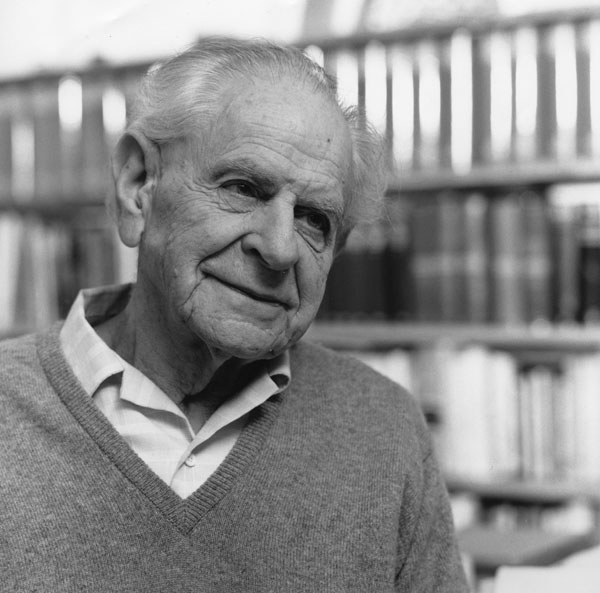
\includegraphics[width=0.65\textwidth]{fig/karl-popper.jpg}
    \caption[Karl Popper]{Porträt von Karl Popper~\cite{PopperPortrait}}
    \label{fig:KarlPopper}
\end{figure}

Karl Popper (siehe auch Abb.~\ref{fig:KarlPopper} auf Seite~\pageref{fig:KarlPopper}) schreibt:

\begin{quote}
"`Wer's nicht einfach und klar sagen kann, der soll schweigen und weiterarbeiten bis er's klar sagen kann."'
\end{quote}

\blindtext

Ein Szenario\footnote{Das ist eine Fußnote.}?

\blindtext

Unter Einbeziehung der Literatur in Kapitel~\ref{chp:LitKrit}, sowie des Gesprächs von Eric Weinstein\footnote{Und eine zweite Fußnote} und Peter Thiel~\cite{WeinsteinThielPortal} \ldots

\blindtext

\blinddescription

\blindtext

\blinditemize

Im Rahmen der Litaraturkritik wurde das Buch (die Bücher) von Byung-Chul Han, \textit{Vom Verschwinden der Rituale}~\cite{HanRituale} gelesen \ldots

Der Podcast zur Vorlesung\footnote{\url{http://podcast.zukunft-denken.eu}} \textit{Zukunft Denken} steht als ergänzende Ressource zur Verfügung.

\blindtext

Scheffer et al beschreiben in ihrem Artikel \ldots ~\cite{SchefferRegimeNature}

\blindtext


%*************************************************************************
%*************************************************************************
\chapter{\LaTeX{} und typographische Anmerkungen} \label{chap:latexRes}

\section{Häufige Fehler} \label{sec:fehler}

\begin{itemize}
    \item \textbf{Spellchecker} nutzen: es wirkt sehr unprofessionell wenn sich Tippfehler etc. im Dokument finden.
    \item Strukturieren des Fließtextes in \textbf{Absätzen}. \textit{Harte Zeilenumbrüche} also \verb+\\+ gibt es im Fließtext niemals. Neuer Absatz in \LaTeX{} wird durch eine Leerzeile zwischen Absätzen ausgelöst.
    \item Absätze werden typographisch auf eine von zwei Möglichkeiten getrennt: mit \textit{Einrückung der ersten Zeile} oder durch \textit{Abstand zwischen den Absätzen}. In der Regel wird ersteres bevorzugt, weil es auch bei Seitenumbrüchen ohne Probleme funktioniert. In \LaTeX{} lässt man schlicht eine Leere Zeile zwischen zwei Absätzen im Quelltext. Das Satzsystem kümmert sich dann um die Typographie des Absatzes. (Keinesfalls aber \verb+\noindent+ oder ähnliches machen.)
    \item Nicht selbst am \textbf{Layout} rumspielen, wenn man sich nicht intensiv mit Typographie beschäftigt hat; z.B. niemals Überschriften mit "`fettem Text"' (also \verb+\textbf{Überschrift}+) machen, sondern die Strukturierung des Dokumentes verwenden.
    \item \textbf{Dokument-Strukturierung} mit: \verb+\part+, \verb+\chapter+, \verb+\section+, \verb+\sub(sub)section+. Die unterste Ebene kann ohne Nummerierung erfolgen: \verb+\paragraph+.
    \item Es gibt \textit{deutsche}, \textit{englische} und \textit{französische} \textbf{Anführungszeichen}. In englischen Texten werden ausschließlich ``englische A'' (\verb+``Text''+) verwendet, im Deutschen "`deutsche"' (\verb+"`Text"'+) oder ">französische As"< (\verb+">Text"<+), niemals englische.
    \item \textbf{Striche} gibt es in drei Arten: Binde-Strich(\verb+-+), 3--4 (\verb+--+) und Gedankenstrich (entweder \verb+---+ bei englischer Typographie oder \verb+ -- + bei deutscher Typographie).
    \item \textbf{Bullet-Punkte} (\verb+\begin{itemize}...\begin{itemize}+ Umgebung) werden für knappe Listen und Aufzählungen verwendet, nicht um Absätze zu strukturieren, dafür verwendet man (sub)sections oder \verb+\paragraph+.
    \item Vorsicht mit \textbf{Satzspiegel-Einstellungen}: (1) richtiges Papierformat wählen (2) Vorsicht mit DIV-Settings. Dieses Template ist vernünftig eingestellt -- im Zweifel diese Einstellungen beibehalten.
    \item \textbf{Zahlen} von 1--12 werden im Deutschen in der Regel ausgeschrieben, also \textit{elf} nicht \textit{11}.
\end{itemize}


\section{Weitere Ressourcen} \label{sec:ressourcen}

\begin{itemize}
    \item \url{https://www.latex-project.org}
    \item \url{https://en.wikibooks.org/wiki/LaTeX}
    \item \url{https://www.overleaf.com}
\end{itemize}




%*************************************************************************
%*************************************************************************
\bibliography{seminararbeit}
\bibliographystyle{plain}

\end{document}
